%% ============================================================
%%  BORRADOR — La Gaceta de la Real Sociedad Matemática Española
%%  Adaptar al fichero de clase oficial de la revista antes del envío
%% ============================================================
\documentclass[11pt,a4paper]{article}

% --- Codificación y lengua ---
\usepackage[utf8]{inputenc}
\usepackage[T1]{fontenc}
\usepackage{lmodern}
% babel spanish not available in this TeX installation
\usepackage{microtype}

% --- Matemáticas ---
\usepackage{amsmath,amsthm,amssymb,amsfonts}
\usepackage{mathtools}

% --- Geometría ---
\usepackage[top=2.5cm,bottom=2.5cm,left=3cm,right=3cm]{geometry}

% --- Gráficos ---
\usepackage{graphicx}
\usepackage{xcolor}
\usepackage{tikz}
\usepackage{tikz-3dplot}
\usetikzlibrary{shadings}
\usepackage{float}
\usepackage{caption}
\usepackage{subcaption}

% --- Código ---
\usepackage{listings}
\lstset{
  basicstyle      = \small\ttfamily,
  keywordstyle    = \color{blue!70!black}\bfseries,
  commentstyle    = \color{green!50!black}\itshape,
  stringstyle     = \color{orange!80!black},
  backgroundcolor = \color{gray!8},
  frame           = single,
  framerule       = 0.4pt,
  rulecolor       = \color{gray!40},
  breaklines      = true,
  columns         = flexible,
  numbers         = none,
  xleftmargin     = 6pt,
  xrightmargin    = 6pt,
}

% --- Tablas ---
\usepackage{booktabs}
\usepackage{array}

% --- Hipervínculos ---
\usepackage[colorlinks=true,
            linkcolor=blue!60!black,
            citecolor=green!40!black,
            urlcolor=blue!70!black]{hyperref}

% --- Entornos matemáticos ---
\theoremstyle{plain}
\newtheorem{teorema}{Teorema}[section]
\newtheorem{proposicion}[teorema]{Proposición}
\newtheorem{corolario}[teorema]{Corolario}
\newtheorem{lema}[teorema]{Lema}

\theoremstyle{definition}
\newtheorem{definicion}[teorema]{Definición}
\newtheorem{ejemplo}[teorema]{Ejemplo}

\theoremstyle{remark}
\newtheorem{observacion}[teorema]{Observación}

% --- Macros ---
\newcommand{\C}{\mathbb{C}}
\newcommand{\R}{\mathbb{R}}
\newcommand{\N}{\mathbb{N}}
\newcommand{\Puno}{\mathbb{P}^1(\mathbb{C})}
\newcommand{\fn}[1]{\texttt{#1}}
\newcommand{\pkg}[1]{\textsl{#1}}
\DeclareMathOperator{\grad}{grado}

% --- Datos del artículo ---
\title{\textbf{Dinámica de funciones racionales en la esfera de Riemann:
       geometría, cuencas de atracción y visualización}}

\author{Víctor Álvarez Aparicio,
        Luis Javier Hernández Paricio
        y María Teresa Rivas Rodríguez\\
        {\small Departamento de Matemáticas y Computación,
        Universidad de La Rioja, Logroño}\\
        {\small \texttt{luis-javier.hernandez@unirioja.es}}}

\date{} % La fecha la pone la revista

% ============================================================
\begin{document}
% ============================================================

\maketitle

\begin{abstract}
Estudiamos la dinámica de iteración de funciones racionales desde la
perspectiva natural de la esfera de Riemann~$\Puno$.
El uso de coordenadas homogéneas elimina el carácter especial del punto
en el infinito y permite ver la dinámica completa: cuencas de atracción
que envuelven la esfera, fronteras fractales que conectan todas las
cartas, y puntos fijos en el infinito que quedan ocultos cuando se
trabaja únicamente en~$\C$.
Ilustramos la teoría con los ejemplos clásicos de Milnor —Newton,
Halley, la familia $z^2+c$— e incluimos la visualización de cuencas
de ciclos periódicos de período~$p\geq 2$, implementada en el paquete
\pkg{RiemannBasins.jl} que acompaña al artículo.
Una parte significativa del trabajo está dedicada al diseño de
visualizaciones inclusivas: describimos criterios matemáticamente
fundados basados en el espacio de color perceptualmente uniforme LCHab
y en la paleta Okabe--Ito, que garantiza que las figuras sean
igualmente legibles para personas con daltonismo.
El código es de libre acceso y reproducible.
\end{abstract}

\bigskip
\noindent\textbf{Palabras clave:} esfera de Riemann, coordenadas homogéneas,
cuencas de atracción, ciclos periódicos, conjunto de Julia, método de Newton,
espacio de color LCHab, visualización inclusiva, daltonismo.

\medskip
\noindent\textbf{MSC 2020:} 37F10, 37F45, 32H50, 68U05.

% ============================================================
\section{Introducción}
% ============================================================

El método de Newton aplicado al polinomio $P(z)=z^3-1$ produce, a partir
de cualquier punto inicial $z_0\in\C$, la sucesión de iterados
\[
   z_{n+1} = z_n - \frac{P(z_n)}{P'(z_n)}
           = \frac{2z_n^3+1}{3z_n^2},
\]
que converge a una de las tres raíces cúbicas de la unidad,
$1,\,\omega=e^{2\pi i/3},\,\omega^2=e^{4\pi i/3}$, según la posición de
$z_0$.
Colorear cada punto $z_0$ según la raíz a la que converge su órbita
produce la figura~\ref{fig:newton_z3}: un fractal con simetría de orden
tres en el que las tres cuencas de atracción se entrelazan de forma
infinitamente intrincada en su frontera común.

\begin{figure}[ht]
  \centering
  % Comando: basin_portrait([1,0,0,-1],[0,3,0,0]; bands=8.0)
  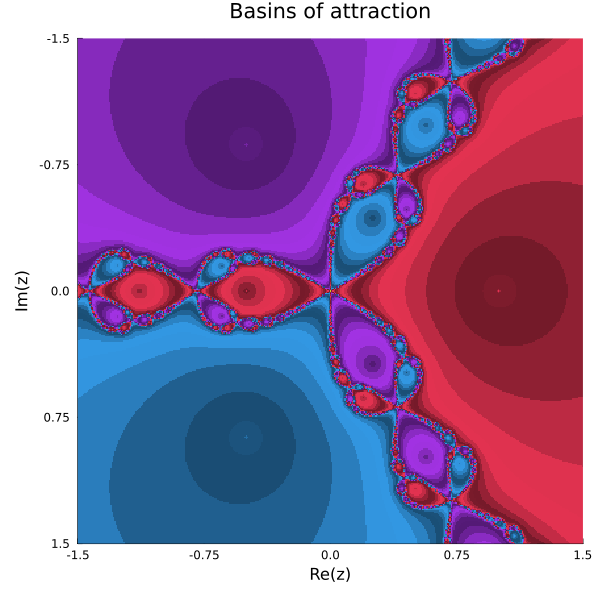
\includegraphics[width=0.55\textwidth]{figures/newton_z3_test.png}
  \caption{Cuencas de atracción del método de Newton para $z^3-1$,
           generadas con la paleta LCHab de \pkg{RiemannBasins.jl}.
           Cada punto se colorea según la raíz a la que converge su
           órbita; los tres tonos tienen luminosidad CIE~$L^*$ idéntica,
           por lo que ninguna cuenca destaca sobre las demás.
           Las bandas concéntricas revelan la velocidad de convergencia
           mediante modulación del canal de luminosidad.}
  \label{fig:newton_z3}
\end{figure}

Esta imagen suscita una pregunta inmediata: ¿qué ocurre con los puntos
que «escapan hacia el infinito»?
En el plano complejo, $\infty$ es una singularidad que se trata de forma
ad hoc.
Sin embargo, para la función racional $f(z)=(2z^3+1)/(3z^2)$, el punto
$\infty$ es también un punto fijo —de hecho, \emph{repulsor}: las órbitas que empiezan cerca de él se alejan, en lugar de converger— con un papel
perfectamente bien definido en la dinámica global.
Verlo requiere salir de~$\C$ y trabajar en su compactificación natural:
la \emph{esfera de Riemann}~$\Puno$.

El presente artículo tiene cuatro objetivos.
El primero es mostrar que $\Puno$, lejos de ser una complicación
abstracta, es el marco más sencillo para estudiar la dinámica de
funciones racionales: elimina los casos especiales ligados al infinito y
hace manifiesta la simetría global de los sistemas.
El segundo es ilustrar la teoría con los ejemplos más iluminadores de la
literatura, en particular los del libro seminal de Milnor~\cite{Milnor2006},
y extenderlos a la visualización de cuencas de ciclos periódicos de
período~$p\geq 2$.
El tercero es describir cómo diseñar visualizaciones matemáticamente
coherentes de las cuencas, usando el espacio de color LCHab (un espacio perceptualmente uniforme derivado del estándar CIE de 1976, descrito en §\ref{sec:visualizacion})
para garantizar que todos los tonos sean perceptualmente equivalentes.
El cuarto —y quizá el menos habitual en la literatura matemática— es
el compromiso con la \emph{inclusión visual}: todas las figuras del
artículo están disponibles también en una paleta accesible para personas
con daltonismo (deuteranopía y protanopía), siguiendo las directrices
de Okabe e~Ito~\cite{OkabeIto2008}.
Con ello, el artículo se suma a la creciente demanda de comunicación
científica accesible para toda la audiencia.

% ============================================================
\section{La esfera de Riemann}
\label{sec:esfera}
% ============================================================

Una \emph{superficie de Riemann} es una superficie (variedad de dimensión
real~2) dotada de un atlas cuyas funciones de cambio de carta son
holomorfas~\cite{Jones1987,Miranda1995}.
Esta condición garantiza que el atlas es internamente consistente en el
sentido complejo: la noción de «función holomorfa sobre la superficie»
tiene el mismo significado con independencia de la carta que se use
para describirla.
Las superficies de Riemann compactas se clasifican topológicamente por su
\emph{género}~$g$ —el número de «asas» de la superficie—: género~$0$
corresponde a la esfera, género~$1$ al toro, etc.

En este artículo nos ocupamos exclusivamente de la única superficie de
Riemann compacta de género~$0$, la \emph{esfera de Riemann}.
Tiene dos realizaciones naturales que conviene conocer en paralelo: una
\emph{geométrica} —la esfera unidad $S^2\subset\R^3$ con proyecciones
estereográficas— y una \emph{algebraica} —el espacio proyectivo complejo
$\Puno$—.
Ambas son el mismo objeto complejo visto desde ángulos distintos, y sus
respectivas ventajas quedarán de manifiesto a lo largo del artículo.

\subsection{La esfera \texorpdfstring{$S^2$}{S2} y las proyecciones estereográficas}

Considere la esfera unidad $S^2\subset\R^3$ con el polo norte $N=(0,0,1)$
y el plano complejo~$\C$ identificado con el plano ecuatorial $\{t=0\}$
(figura~\ref{fig:stereo}).
Dado un punto $(x,y,t)\in S^2\setminus\{N\}$,
trace la semirrecta que parte de~$N$ y pasa por $(x,y,t)$; esa semirrecta
corta al plano ecuatorial en un único punto complejo~$z$.
Esta construcción es la \emph{proyección estereográfica desde el polo norte}:
\[
  z = \frac{x+iy}{1-t}\;\in\;\C,
\]
con fórmula inversa
\[
   (x,y,t) = \left(\frac{2\operatorname{Re}(z)}{|z|^2+1},\;
                    \frac{2\operatorname{Im}(z)}{|z|^2+1},\;
                    \frac{|z|^2-1}{|z|^2+1}\right).
\]

\begin{figure}[ht]
\centering
\tdplotsetmaincoords{70}{120}
\begin{tikzpicture}[tdplot_main_coords, scale=1.8, font=\small, >=stealth]

  %% ── Plano ecuatorial (dibujado primero, detrás de la esfera) ─────────────
  \fill[blue!8, opacity=0.70]
      (-1.5,-1.3,0) -- (2.1,-1.3,0) -- (2.1,1.9,0) -- (-1.5,1.9,0) -- cycle;
  \draw[blue!35!black, thin]
      (-1.5,-1.3,0) -- (2.1,-1.3,0) -- (2.1,1.9,0) -- (-1.5,1.9,0) -- cycle;
  \node[blue!55!black] at (2.25,0.2,0) {$\mathbb{C}$};

  %% ── Meridiano oculto (azimut 60°, semiciclo trasero) ─────────────────────
  \tdplotsetthetaplanecoords{60}
  \tdplotdrawarc[tdplot_rotated_coords, gray!30, dashed, thin]%
      {(0,0,0)}{1}{180}{360}{}{}

  %% ── Semiciclo ecuatorial oculto ──────────────────────────────────────────
  %% Vista desde azimut 120°: oculto de 30° a 210°
  \tdplotdrawarc[black!70, dashed]{(0,0,0)}{1}{120}{300}{}{}

  %% ── Cuerpo de la esfera (ball shading en coordenadas de pantalla) ─────────
  \shade[tdplot_screen_coords, ball color=gray!15, opacity=0.45] (0,0) circle (1);
  \draw[tdplot_screen_coords, gray!65, thin] (0,0) circle (1);

  %% ── Meridiano visible (azimut 60°, semiciclo delantero) ──────────────────
  \tdplotsetthetaplanecoords{60}
  \tdplotdrawarc[tdplot_rotated_coords, gray!45, thin]%
      {(0,0,0)}{1}{0}{180}{}{}

  %% ── Semiciclo ecuatorial visible (delantero) ─────────────────────────────
  %% Vista desde azimut 120°: visible de -150° a 30°
  \tdplotdrawarc[black, thick]{(0,0,0)}{1}{-60}{120}{}{}

  %% ── Eje vertical ─────────────────────────────────────────────────────────
  \draw[gray!50, thin] (0,0,0) -- (0,0,1.28);
  \draw[gray!35, dashed, thin] (0,0,-1.1) -- (0,0,0);

  %% ── Polos ────────────────────────────────────────────────────────────────
  \fill (0,0,1)  circle (0.9pt) node[above=2pt] {$N$};
  \fill (0,0,-1) circle (0.9pt) node[below=2pt]  {$S$};

  %% ── Semirrecta de proyección ─────────────────────────────────────────────
  %% P=(sin60°cos60°, sin60°sin60°, cos60°)=(0.433, 0.750, 0.500) ∈ S²
  %% z_proy = (x/(1−t), y/(1−t), 0) = (0.866, 1.500, 0)
  \coordinate (Npt) at (0,0,1);
  \coordinate (Ppt) at (0.433,0.750,0.500);
  \coordinate (Zpt) at (0.866,1.500,0);

  \draw[red!70!black, dashed, thick] (Npt) -- (Zpt);

  \fill[red!65!black] (Ppt) circle (1.2pt);
  \node[right=3pt, red!65!black] at (Ppt) {$P\!=\!(x,y,t)$};

  \fill[blue!65!black] (Zpt) circle (1.2pt);
  \node[above right=2pt, blue!65!black] at (Zpt) {$z$};

\end{tikzpicture}
\caption{Proyección estereográfica desde el polo norte~$N$.
         La semirrecta que parte de~$N$ y pasa por $P=(x,y,t)\in S^2$
         corta al plano ecuatorial~$\mathbb{C}$ en el punto $z=(x+iy)/(1-t)$.}
\label{fig:stereo}
\end{figure}

Esta primera carta $(U_0, z)$, con $U_0 = S^2\setminus\{N\}$, cubre toda
la esfera salvo~$N$; el polo norte actúa como «punto en el infinito» de
la carta afín~$z$.

Para cubrir también~$N$ se necesita una segunda carta en su entorno.
La elección más directa sería proyectar desde el polo sur~$S$,
obteniendo la coordenada
\[
  \tilde{w} = \frac{x+iy}{1+t}\;\in\;\C.
\]
Sin embargo, el cambio de carta entre~$z$ y~$\tilde{w}$ resulta ser
$\tilde{w} = 1/\bar{z}$, que involucra la conjugación compleja y
no es holomorfo (es \emph{anti}holomorfo).
Para remediar esto basta componer con la reflexión $w=\overline{\tilde{w}}$,
obteniendo la segunda carta $(U_1, w)$, con $U_1 = S^2\setminus\{S\}$:
\[
  w = \frac{x-iy}{1+t}\;\in\;\C,
\]
cuyo cambio de carta con~$z$ en la región de solapamiento $U_0\cap U_1$ es
simplemente
\[
  w \;=\; \frac{1}{z},
\]
perfectamente holomorfo.
Con estas dos cartas, $S^2$ tiene estructura de superficie de Riemann.

\begin{observacion}
La proyección estereográfica es \emph{conforme}: preserva los ángulos
entre curvas, aunque no las distancias.
Una consecuencia notable es que los círculos y rectas del plano se
corresponden exactamente con los círculos de~$S^2$, propiedad fundamental
en la teoría de las transformaciones de Möbius~\cite{Needham1997}.
\end{observacion}

\subsection{El espacio proyectivo \texorpdfstring{$\Puno$}{P1(C)}}

La segunda realización prescinde de~$\R^3$ y trabaja directamente con
pares de números complejos.
El \emph{espacio proyectivo complejo unidimensional}~$\Puno$ es el conjunto
de rectas complejas que pasan por el origen de~$\C^2$:
\[
  \Puno = \bigl(\C^2\setminus\{(0,0)\}\bigr)\,\big/\!\sim,
  \qquad
  (z_0,z_1)\sim(\lambda z_0,\lambda z_1)\;\forall\,\lambda\in\C^*.
\]
La clase de $(z_0,z_1)$ se escribe $[z_0:z_1]$ y se llama \emph{punto
homogéneo}; en cada clase solo importa el cociente $z_0/z_1$,
no los valores individuales.

$\Puno$ se cubre con dos cartas afines:
\begin{align*}
  U_0 &= \{[z_0:z_1]\;:\;z_1\neq 0\},
  &z &= z_0/z_1\;\in\;\C,\\
  U_1 &= \{[z_0:z_1]\;:\;z_0\neq 0\},
  &w &= z_1/z_0\;\in\;\C,
\end{align*}
con cambio de carta $w=1/z$ en $U_0\cap U_1$ —idéntico al obtenido
con las proyecciones estereográficas—, lo que confirma que ambas
construcciones definen la misma superficie de Riemann: $\Puno\cong\hat{\C}$.

La ventaja de~$\Puno$ frente a~$\hat{\C}$ es de simetría: ningún punto
ocupa un lugar especial.
El «punto en el infinito» de la carta~$z$ es simplemente $[1:0]\in U_1$,
con coordenada $w=0$ en la carta~$w$, y se trata exactamente igual que
cualquier otro punto.
Esta simetría resulta esencial cuando se estudian funciones racionales,
como veremos en la sección siguiente.

% ============================================================
\section{Funciones racionales en \texorpdfstring{$\Puno$}{P1(C)}}
\label{sec:racionales}
% ============================================================

\subsection{Extensión natural al espacio proyectivo}

Una \emph{función racional} $f:\C\to\hat{\C}$ se escribe
$f(z)=p(z)/q(z)$ con $p,q$ polinomios sin factor común.
Su \emph{grado} es $d=\max(\deg p,\deg q)$.
Para extenderla a $\Puno$ de forma regular —incluyendo el punto en el
infinito— se homogenizan el numerador y el denominador:
\[
  P(z_0,z_1) = z_1^d\,p\!\left(\tfrac{z_0}{z_1}\right),\qquad
  Q(z_0,z_1) = z_1^d\,q\!\left(\tfrac{z_0}{z_1}\right).
\]
Ambos son polinomios homogéneos de grado~$d$, y la aplicación
\[
  F:\Puno\longrightarrow\Puno,\qquad
  [z_0:z_1]\longmapsto [P(z_0,z_1):Q(z_0,z_1)]
\]
está bien definida (el cociente $[P:\!Q]$ no depende del representante)
y es holomorfa.
En la carta afín $z=z_0/z_1$ recuperamos $f(z)=p(z)/q(z)$; en la carta
$w=z_1/z_0$ la función toma la forma regular $\tilde{f}(w)$ sin polos.

\begin{ejemplo}[Newton para $z^3-1$]
$f(z)=(2z^3+1)/(3z^2)$, de grado~$3$.
Homogeneizando con $d=3$:
$P(z_0,z_1)=2z_0^3+z_1^3$,\; $Q(z_0,z_1)=3z_0^2 z_1$.
En la carta $w$:
\[
   \tilde{f}(w) = \frac{3w}{2+w^3},\qquad\tilde{f}(0)=0,\qquad
   \tilde{f}'(0)=\tfrac{3}{2}.
\]
El punto $[1:0]$ (infinito en la carta $z$) tiene imagen $[1:0]$ y
derivada~$\tilde{f}'(0)=3/2>1$: es un \emph{punto fijo repulsor}
(el concepto de \emph{multiplicador} se precisa en la sección~\ref{sec:pfijos}).
\end{ejemplo}

\subsection{Puntos fijos y su multiplicador}
\label{sec:pfijos}

Un \emph{punto fijo} de $f$ en $\Puno$ es un punto $\zeta$ con
$f(\zeta)=\zeta$.
Para un punto fijo finito $\zeta\in\C$, el \emph{multiplicador} es
$\lambda=f'(\zeta)\in\C$.
Para el punto $\zeta=\infty$, se usa la carta $w=1/z$: el multiplicador
es la derivada de $\tilde{f}$ en $w=0$.

La interpretación geométrica es sencilla: si se toma un disco pequeño
$D(\zeta,\varepsilon)$ de radio $\varepsilon$ centrado en el punto fijo~$\zeta$,
su imagen $f(D(\zeta,\varepsilon))$ es aproximadamente un disco de radio
$|\lambda|\,\varepsilon$ centrado en~$\zeta$ (pues $f(\zeta)=\zeta$),
girado un ángulo $\arg\lambda$ respecto al original.
El módulo~$|\lambda|$ es, pues, el factor de escala local:
si $|\lambda|<1$ el disco se contrae iteración tras iteración y
los puntos cercanos convergen a~$\zeta$;
si $|\lambda|>1$ el disco se expande y $\zeta$ repele a sus vecinos.

El caso límite $\lambda=0$ —denominado punto fijo \emph{superatractor}— es cualitativamente distinto.
Cuando $\lambda=0$ la aproximación lineal colapsa y la dinámica local
la gobierna el primer término no nulo de la expansión de Taylor:
si $f(z)\approx\zeta+a_k(z-\zeta)^k$ con $a_k\neq 0$ y $k\geq 2$,
entonces el disco $D(\zeta,\varepsilon)$ se lleva sobre un disco imagen de
radio $\approx|a_k|\,\varepsilon^k\ll\varepsilon$, pero de manera \emph{$k$ a~$1$}:
el disco original se <<enrolla>> $k$ veces sobre la imagen,
como una hoja que se pliega sobre sí misma.
La convergencia es de orden~$k$ (cuadrática si $k=2$), mucho más rápida
que la lineal de los atractores ordinarios.
En particular, las raíces simples de un polinomio~$P$ son siempre puntos
fijos superatractores del método de Newton $f=N_P$, con $k=2$.

La clasificación por el módulo del multiplicador es la habitual:
\begin{itemize}
  \item $|\lambda|<1$: punto fijo \emph{atractor}; el caso especial $\lambda=0$ es el \emph{superatractor} descrito arriba.
  \item $|\lambda|=1$: punto fijo \emph{indiferente}.
  \item $|\lambda|>1$: punto fijo \emph{repulsor}.
\end{itemize}

El siguiente resultado es uno de los más elegantes de la teoría:

\begin{teorema}[Conteo de puntos fijos en $\Puno$]
\label{teo:puntosfijos}
Una función racional de grado $d\geq 1$ tiene exactamente $d+1$
puntos fijos en~$\Puno$, contados con multiplicidad.
\end{teorema}

\begin{proof}[Demostración (esquema)]
Los puntos fijos son las soluciones de $F([z_0:z_1])=[z_0:z_1]$,
es decir, $[P(z_0,z_1):Q(z_0,z_1)]=[z_0:z_1]$.
Esto equivale a $z_1 P(z_0,z_1)-z_0 Q(z_0,z_1)=0$, un polinomio
homogéneo de grado $d+1$, que por el teorema de Bézout proyectivo
tiene exactamente $d+1$ raíces (con multiplicidad) en~$\Puno$.
\end{proof}

Para el método de Newton de un polinomio $P$ de grado $n$, la función
$f$ tiene grado $n$, sus $n$ puntos fijos finitos son exactamente
las raíces de~$P$ (todas superatractoras, pues $f'(\zeta)=0$ en toda
raíz simple), y el punto en el infinito es el $n+1$-ésimo punto fijo.

% ============================================================
\section{Cuencas de atracción y conjuntos de Julia}
\label{sec:cuencas}
% ============================================================

\subsection{Conjuntos de Fatou y de Julia}
\label{ssec:julia}

Dada una función racional $f:\Puno\to\Puno$ de grado $d\geq 2$,
definimos el \emph{conjunto de Fatou} $\mathcal{F}(f)$ como el mayor
abierto de $\Puno$ en el que la familia de iterados
$\{f^n\}_{n\geq 1}$ es una \emph{familia normal} en el sentido de Montel (es decir, equicontinua: pequeñas perturbaciones del punto de partida producen pequeñas perturbaciones de la órbita completa).
Su complementario $\mathcal{J}(f)=\Puno\setminus\mathcal{F}(f)$ es el
\emph{conjunto de Julia}.

Intuitivamente, $\mathcal{F}(f)$ es la región de dinámica estable
—pequeñas perturbaciones del punto inicial producen pequeñas
perturbaciones de la órbita—, mientras que $\mathcal{J}(f)$ es la
región de dinámica caótica, donde la sensibilidad a las condiciones
iniciales es máxima.

\medskip
\noindent\textbf{¿Qué significa «familia normal»?}
La idea, antes de la definición precisa, es la siguiente: imagina
observar $n$ iteraciones sucesivas de $f$ desde un punto $z$.
Si perturbar ligeramente $z$ cambia poco el resultado final para todo~$n$,
la dinámica es predecible —estamos en $\mathcal{F}(f)$—.
Si, en cambio, perturbaciones diminutas producen resultados completamente
distintos para algún $n$ grande, la dinámica es impredecible:
estamos en $\mathcal{J}(f)$.

Formalmente, una familia $\mathcal{G}=\{g_\alpha\}$ de funciones holomorfas
en un abierto $U\subset\Puno$ es \emph{normal} si de toda sucesión
$g_{\alpha_n}\subset\mathcal{G}$ puede extraerse una subsucesión que
converge uniformemente en compactos de~$U$ —bien a una función holomorfa,
bien a la constante $\infty$—.
El criterio de Montel hace esto practicable: basta con que todas las
funciones de $\mathcal{G}$ eviten simultáneamente dos valores fijos
$a,b\in\Puno$ para garantizar la normalidad.

\medskip
\noindent\textbf{Generalización a familias más amplias.}
En la definición clásica la familia es $\mathcal{G}=\{f^n:n\geq 1\}$,
los iterados de una sola función.
Pero la misma noción se extiende de forma natural, de menos a más general:

\begin{itemize}
  \item \textbf{Sucesiones no estacionarias.}
        Si en cada paso se aplica una función (posiblemente distinta) de
        una familia prefijada $\{f_1,f_2,\ldots\}$, se obtiene una
        \emph{sucesión de composiciones}
        $h_n = f_{i_n}\circ\cdots\circ f_{i_1}$.
        El conjunto de Fatou de la familia es el mayor abierto donde
        todas estas sucesiones forman una familia normal,
        independientemente de cómo se elijan los índices.
  \item \textbf{Semigrupos racionales.}
        Dadas $f$ y $g$ racionales de grado $\geq 2$, el
        \emph{semigrupo} $\langle f,g\rangle$ consta de todas las
        composiciones finitas con exponentes no negativos.
        La teoría de Fatou-Julia del semigrupo —iniciada por
        Hinkkanen y Martin— define $\mathcal{F}(\langle f,g\rangle)$
        como el mayor abierto donde toda la familia de composiciones
        es normal; su complementario puede ser mucho más complejo
        que el Julia de cada función por separado.
  \item \textbf{Grupos kleinianos.}
        Si $f$ y $g$ son transformaciones de Möbius (grado~$1$),
        generan un grupo $\langle f,g\rangle\leq\mathrm{Aut}(\Puno)$.
        El conjunto de Fatou del grupo es el mayor abierto donde la
        familia de \emph{todas} las palabras $f^{\pm 1},g^{\pm 1},\ldots$
        es normal; su complementario es el \emph{conjunto límite}
        del grupo kleiniano, análogo del conjunto de Julia.
\end{itemize}

Ambas generalizaciones conectan directamente con las perspectivas
descritas en la sección~\ref{sec:conclusion}.

\begin{proposicion}[Propiedades del conjunto de Julia]
$\mathcal{J}(f)$ es compacto, no vacío, perfectamente invariante
($f^{-1}(\mathcal{J})=\mathcal{J}=f(\mathcal{J})$), y es la
adherencia del conjunto de puntos periódicos repulsores.
\end{proposicion}

\subsection{Cuencas de atracción}

La \emph{cuenca de atracción inmediata} de un punto fijo atractor
$\zeta$ es
\[
  \mathcal{A}^*(\zeta)=\{z\in\Puno\;:\;f^n(z)\to\zeta,\;
  f^n(z)\text{ permanece cerca de }\zeta\}.
\]
La \emph{cuenca de atracción total} $\mathcal{A}(\zeta)$ incluye
además todas las preimágenes iteradas de $\mathcal{A}^*(\zeta)$.
Un resultado fundamental de Fatou garantiza que $\mathcal{A}^*(\zeta)$
es simplemente conexo si el punto crítico de $f$ más cercano cae en~$\mathcal{A}^*(\zeta)$.

La frontera de cada cuenca de atracción es precisamente el conjunto
de Julia $\mathcal{J}(f)$.
En los ejemplos del método de Newton, $\mathcal{J}(f)$ separa las
cuencas de las distintas raíces: su geometría fractal —habitualmente
de dimensión de Hausdorff estrictamente entre 1 y 2— es la que produce
las imágenes más llamativas.

\subsection{Clasificación de los componentes de Fatou}

Un resultado central de la teoría —el \emph{teorema de clasificación de Fatou--Sullivan}~\cite{Milnor2006}, cuya demostración requiere herramientas profundas de variable compleja que van más allá del alcance de este artículo— establece que todo
componente periódico del conjunto de Fatou es de uno de estos cinco
tipos:

\begin{enumerate}
  \item \textbf{Cuenca de atractor fijo:} $f^n(z)\to\zeta$ con $|\lambda|<1$.
  \item \textbf{Cuenca de ciclo atractor:} $f^{np}(z)\to\zeta_j$ donde
        $\{\zeta_1,\ldots,\zeta_p\}$ es un ciclo de período $p\geq 2$.
  \item \textbf{Cuenca parabólica:} convergencia a un punto fijo de
        multiplicador $\lambda=e^{2\pi i r}$, $r\in\mathbb{Q}$.
  \item \textbf{Disco de Siegel:} componente simplemente conexo con
        dinámica de rotación irracional.
  \item \textbf{Anillo de Herman:} componente doblemente conexo (topología de corona)
        con dinámica de rotación irracional.
\end{enumerate}

\begin{figure}[htbp]
\centering
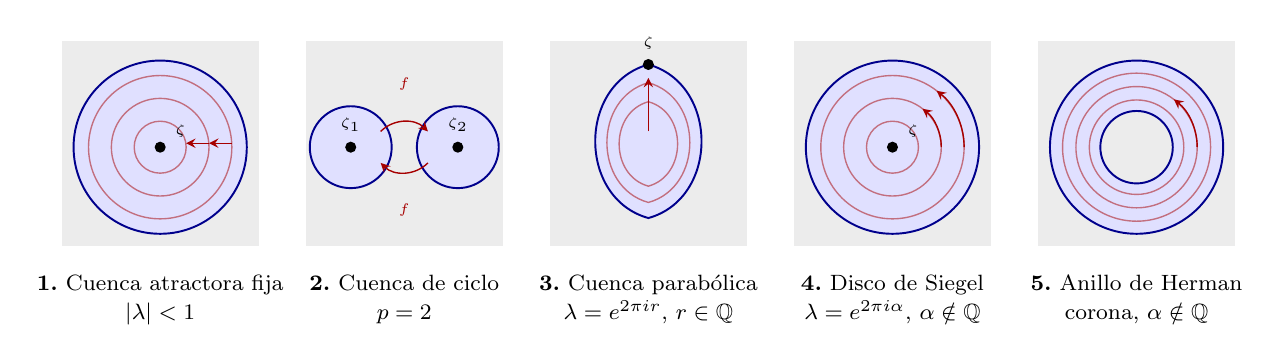
\begin{tikzpicture}[scale=1, font=\footnotesize, >=stealth,
    basin/.style={fill=blue!12, draw=blue!55!black, line width=0.7pt},
    orbit/.style={red!65!black, line width=0.5pt},
    fp/.style={fill=black, circle, minimum size=4pt, inner sep=0pt}
  ]

  %% ===== 1. Cuenca de atractor fijo (centro en x=0) =====
  \begin{scope}[xshift=0cm]
    \fill[gray!15] (-1.25,-1.25) rectangle (1.25,1.35);
    \fill[basin] (0,0) circle (1.1);
    \foreach \r in {0.33,0.62,0.91}
      \draw[orbit, opacity=0.5] (0,0) circle (\r);
    \draw[->, orbit] (0.91,0.05) -- (0.62,0.05);
    \draw[->, orbit] (0.62,0.05) -- (0.33,0.05);
    \node[fp] at (0,0) {};
    \node[above right, font=\tiny] at (0.07,0) {$\zeta$};
    \node[below, align=center] at (0,-1.5)
      {\textbf{1.}\ Cuenca atractora fija\\[1pt]$|\lambda|<1$};
  \end{scope}

  %% ===== 2. Cuenca de ciclo p=2 (centro en x=3.1) =====
  \begin{scope}[xshift=3.1cm]
    \fill[gray!15] (-1.25,-1.25) rectangle (1.25,1.35);
    \fill[basin] (-0.68,0) circle (0.52);
    \fill[basin] ( 0.68,0) circle (0.52);
    \node[fp] at (-0.68,0) {};
    \node[fp] at ( 0.68,0) {};
    \node[above=2pt, font=\tiny] at (-0.68,0) {$\zeta_1$};
    \node[above=2pt, font=\tiny] at ( 0.68,0) {$\zeta_2$};
    \draw[->, orbit] (-0.30, 0.20) to[bend left=45] (0.30, 0.20);
    \draw[->, orbit] ( 0.30,-0.20) to[bend left=45] (-0.30,-0.20);
    \node[above, orbit, font=\tiny] at (0, 0.60) {$f$};
    \node[below, orbit, font=\tiny] at (0,-0.60) {$f$};
    \node[below, align=center] at (0,-1.5)
      {\textbf{2.}\ Cuenca de ciclo\\[1pt]$p=2$};
  \end{scope}

  %% ===== 3. Cuenca parabólica (centro en x=6.2) =====
  \begin{scope}[xshift=6.2cm]
    \fill[gray!15] (-1.25,-1.25) rectangle (1.25,1.35);
    % Petalo: forma suave con la punta en la parte superior (punto fijo en la frontera)
    \fill[basin]
      (0,1.05) .. controls (0.90,0.80) and (0.90,-0.65) .. (0,-0.90)
               .. controls (-0.90,-0.65) and (-0.90,0.80) .. cycle;
    % Curvas de nivel anidadas que convergen al punto parabolico
    \foreach \s in {0.55, 0.78}
      \draw[orbit, opacity=0.5]
        (0,\s*1.05) .. controls (\s*0.90,\s*0.80) and (\s*0.90,-\s*0.65) .. (0,-\s*0.90)
                    .. controls (-\s*0.90,-\s*0.65) and (-\s*0.90,\s*0.80) .. cycle;
    \draw[->, orbit] (0,0.20) -- (0,0.88);
    % Punto fijo parabolico (en la FRONTERA del componente)
    \node[fp] at (0,1.05) {};
    \node[above=2pt, font=\tiny] at (0,1.05) {$\zeta$};
    \node[below, align=center] at (0,-1.5)
      {\textbf{3.}\ Cuenca parab\'olica\\[1pt]$\lambda=e^{2\pi ir}$,\ $r\in\mathbb{Q}$};
  \end{scope}

  %% ===== 4. Disco de Siegel (centro en x=9.3) =====
  \begin{scope}[xshift=9.3cm]
    \fill[gray!15] (-1.25,-1.25) rectangle (1.25,1.35);
    \fill[basin] (0,0) circle (1.1);
    \foreach \r in {0.33,0.62,0.91}
      \draw[orbit, opacity=0.5] (0,0) circle (\r);
    % Flechas de ROTACION (no convergentes)
    \draw[->, orbit] (0.91,0) arc[start angle=0, end angle=52, radius=0.91];
    \draw[->, orbit] (0.62,0) arc[start angle=0, end angle=52, radius=0.62];
    \node[fp] at (0,0) {};
    \node[above right, font=\tiny] at (0.07,0) {$\zeta$};
    \node[below, align=center] at (0,-1.5)
      {\textbf{4.}\ Disco de Siegel\\[1pt]$\lambda=e^{2\pi i\alpha}$,\ $\alpha\notin\mathbb{Q}$};
  \end{scope}

  %% ===== 5. Anillo de Herman (centro en x=12.4) =====
  \begin{scope}[xshift=12.4cm]
    \fill[gray!15] (-1.25,-1.25) rectangle (1.25,1.35);
    % Corona: disco exterior relleno de azul, agujero interior en gris
    \fill[blue!12] (0,0) circle (1.1);
    \fill[gray!15] (0,0) circle (0.46);
    \draw[blue!55!black, line width=0.7pt] (0,0) circle (1.1);
    \draw[blue!55!black, line width=0.7pt] (0,0) circle (0.46);
    % Circulos concentricos invariantes en la corona
    \foreach \r in {0.60,0.77,0.94}
      \draw[orbit, opacity=0.5] (0,0) circle (\r);
    \draw[->, orbit] (0.77,0) arc[start angle=0, end angle=52, radius=0.77];
    \node[below, align=center] at (0,-1.5)
      {\textbf{5.}\ Anillo de Herman\\[1pt]corona,\ $\alpha\notin\mathbb{Q}$};
  \end{scope}

\end{tikzpicture}
\caption{Esquema de los cinco tipos de componentes peri\'odicos del conjunto de Fatou
(teorema de Fatou--Sullivan).
Azul: componente del conjunto de Fatou; gris: complemento
(conjunto de Julia y otros componentes).
Los trazos rojos ilustran la din\'amica interna de cada componente:
curvas de nivel convergentes al punto fijo (casos 1 y~3),
flechas de la aplicaci\'on $f$ entre los puntos del ciclo (caso~2)
y curvas invariantes bajo rotaci\'on irracional (casos 4 y~5).
En el caso~3 el punto fijo parab\'olico~$\zeta$ est\'a en la \emph{frontera} del componente;
en los casos~1 y~4 est\'a en el interior.}
\label{fig:fatou-tipos}
\end{figure}


Para el método de Newton de un polinomio, solo aparecen cuencas del
tipo~(i) —las raíces son superatractoras— y eventualmente del tipo~(iii)
para polinomios con raíces múltiples.
Los tipos~(iv) y~(v) requieren funciones racionales con propiedades
aritméticas muy especiales en los multiplicadores.

% ============================================================
\section{Ejemplos clásicos}
\label{sec:ejemplos}
% ============================================================

\subsection{Newton para \texorpdfstring{$z^3-1$}{z3-1}: el ejemplo fundamental}

Como ya vimos, $f(z)=(2z^3+1)/(3z^2)$ tiene grado 3 y cuatro puntos
fijos en~$\Puno$: las tres raíces cúbicas de la unidad (superatractoras)
y el infinito (repulsor con multiplicador~$3/2$).

Por el Teorema~\ref{teo:puntosfijos}, $3+1=4$ puntos fijos, y efectivamente
los encontramos todos.
La simetría del sistema bajo la rotación $z\mapsto\omega z$ garantiza
que las tres cuencas tienen exactamente la misma forma, rotadas entre
sí $120^\circ$.

La frontera entre las cuencas —el conjunto de Julia $\mathcal{J}(f)$—
tiene una propiedad sorprendente conocida desde Fatou (1919): \emph{en
todo punto de la frontera de una cuenca se acumulan puntos de las otras
dos cuencas}.
Esto implica que los tres colores aparecen simultáneamente en cualquier
ampliación arbitraria de la frontera.

\begin{figure}[ht]
  \centering
  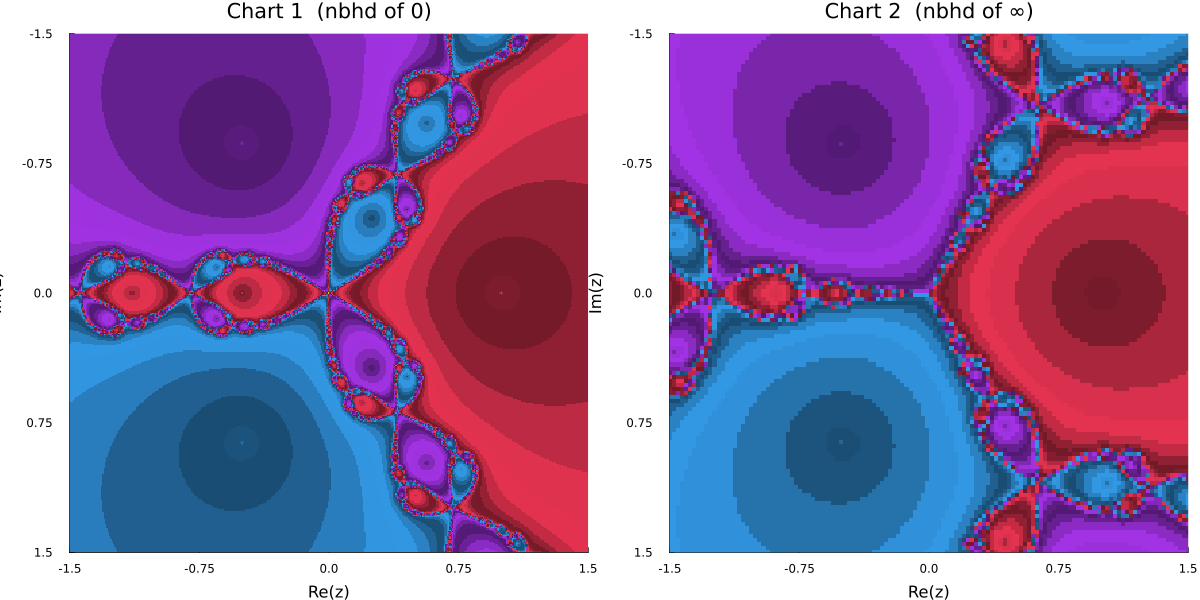
\includegraphics[width=0.90\textwidth]{figures/newton_two_charts.png}
  \caption{Newton para $z^3-1$ en las dos cartas de $\Puno$.
           La carta afín estándar (izquierda) muestra las tres cuencas
           con simetría ternaria.
           La segunda carta estereográfica (derecha) revela que el punto
           en el infinito es repulsor y queda en la frontera de las tres
           cuencas, oculto en la representación plana habitual.
           Generado con \pkg{RiemannBasins.jl}.}
  \label{fig:newton_z3_doble}
\end{figure}

\subsection{Newton para \texorpdfstring{$z^4-1$}{z4-1}: el infinito como cuenca}

Para $P(z)=z^4-1$, el método de Newton da
\[
  f(z)=\frac{3z^4+1}{4z^3},\quad d=4,
\]
con cinco puntos fijos en $\Puno$: las cuatro raíces cuartas de la
unidad ($1,i,-1,-i$, todas superatractoras) y el infinito.

Ahora la imagen de $f$ en la segunda carta $w=1/z$ es
$\tilde{f}(w)=4w/(3+w^4)$,
con $\tilde{f}(0)=0$ y $\tilde{f}'(0)=4/3$.
El punto en el infinito es de nuevo repulsor (multiplicador~$4/3$).

\begin{figure}[ht]
  \centering
  % Comando: two_chart_portrait([1,0,0,0,3],[0,0,0,4,0]; bands=8.0, savepath="figures/newton_z4_two_charts.png")
  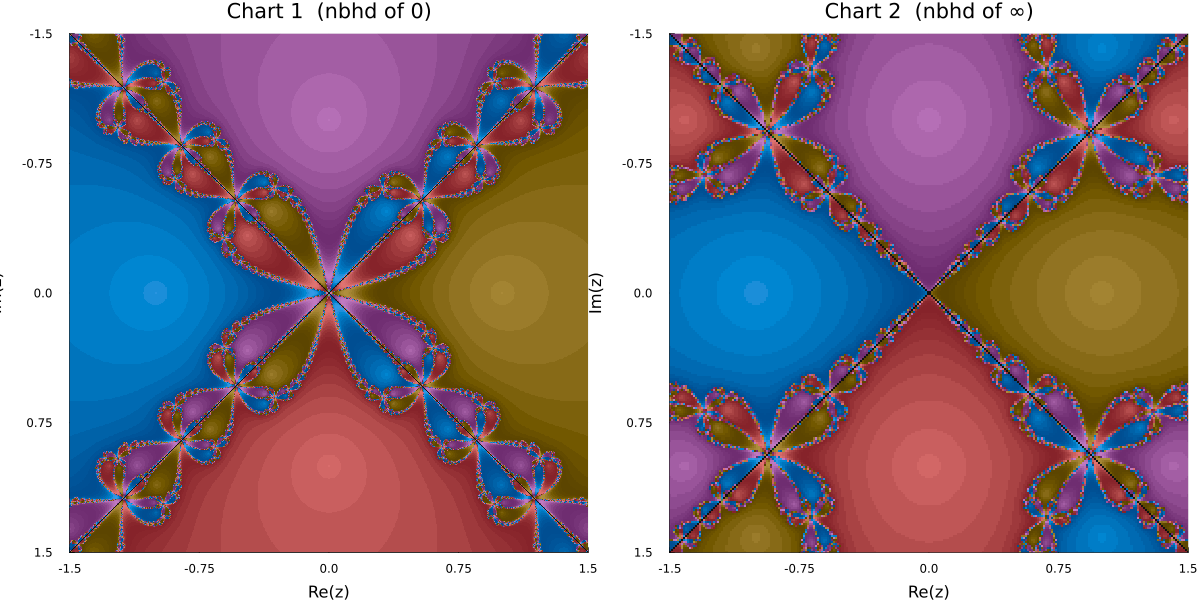
\includegraphics[width=0.90\textwidth]{figures/newton_z4_two_charts.png}
  \caption{Newton para $z^4-1$ en las dos cartas de $\Puno$ (carta~1 a la izquierda, carta~2 a la derecha).
           En la segunda carta se aprecia la cuenca que rodea el punto en
           el infinito (repulsor), oculta en la representaci\'{o}n plana
           habitual.
           Generado con el paquete \pkg{RiemannBasins.jl}.}
  \label{fig:newton_z4}
\end{figure}

La segunda carta revela la estructura global de la dinámica: las cuatro
cuencas se distribuyen simétricamente en torno al repulsor en el
infinito, y la frontera fractal tiene simetría de orden cuatro.
Esta imagen es imposible de obtener si se trabaja únicamente en~$\C$.

\subsection{El método de Halley}

El \emph{método de Halley} para el polinomio $P$ es el esquema de orden
cúbico
\[
   z_{n+1} = z_n - \frac{2P(z_n)P'(z_n)}{2[P'(z_n)]^2-P(z_n)P''(z_n)}.
\]
Aplicado a $P(z)=z^3-1$, produce una función racional de grado~5 cuyos
puntos fijos finitos son también las raíces de~$P$, pero las cuencas
de atracción son más «anchas» y la frontera fractal, aunque sigue siendo
el conjunto de Julia, tiene una geometría diferente a la del método de
Newton.

\begin{figure}[ht]
  \centering
  % Comando: two_chart_portrait(halley_num, halley_den; bands=8.0)
  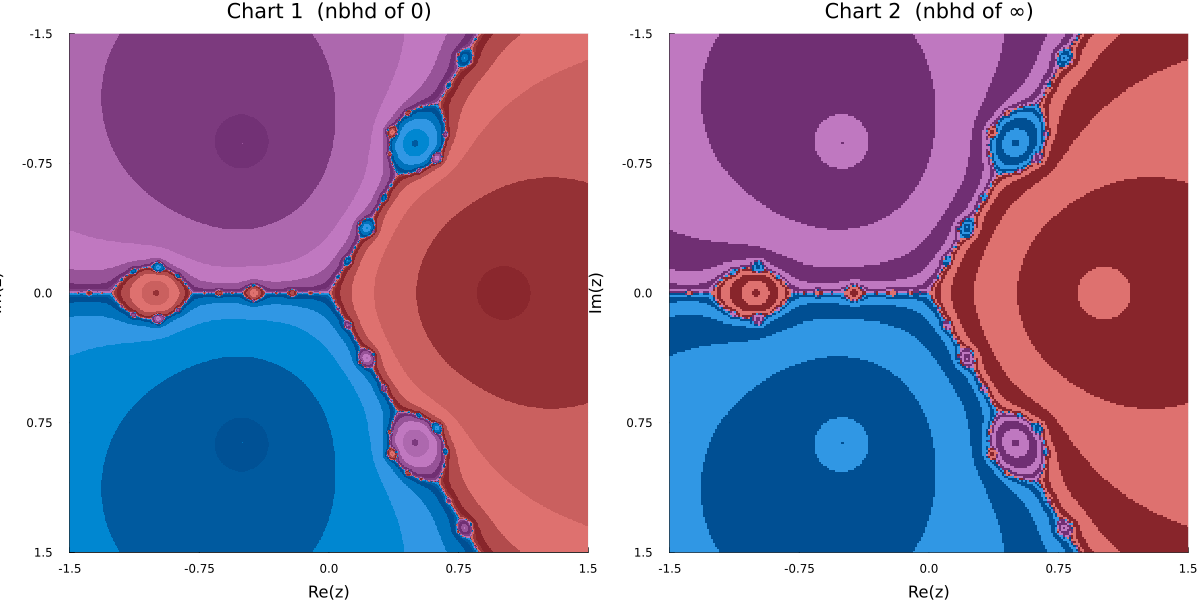
\includegraphics[width=0.75\textwidth]{figures/halley_z3_two_charts.png}
  \caption{Método de Halley para $z^3-1$ en las dos cartas de $\Puno$.
           Las cuencas son más regulares que en Newton y la frontera
           fractal es más suave.}
  \label{fig:halley}
\end{figure}

La comparación entre Newton y Halley ilustra cómo distintos métodos
numéricos para un mismo problema producen estructuras topológicas
globalmente diferentes en~$\Puno$, aunque compartan las mismas
cuencas de atracción finales.

\subsection{Una familia de Milnor: \texorpdfstring{$z^2+c$}{z2+c}}

Las funciones $f_c(z)=z^2+c$ con $c\in\C$ son el ejemplo prototípico
de la teoría de polinomios de Milnor.
Para ciertos valores de~$c$, la órbita del punto crítico $z=0$ converge
a un ciclo atractor de período~$p$, dando lugar a cuencas de una
complejidad topológica creciente.

\begin{itemize}
  \item $c=0$: $f_0(z)=z^2$, cuenca de atracción de $0$ es el disco
        unitario; cuenca de atracción de $\infty$ es el exterior.
  \item $c=-1$: existe un ciclo atractor $\{0,-1\}$ de período~2.
        La cuenca tiene una estructura de «conejo de Douady».
  \item $c=-2$: $f_{-2}$ tiene un punto de Julia real ($[-2,2]$);
        cuencas de $\pm\infty$ son todo el complementario.
\end{itemize}

En todos los casos, $\infty$ es un punto fijo superatractor de la
extensión a $\Puno$: la cuenca del infinito es la componente de Fatou
exterior, que en la segunda carta estereográfica aparece como la cuenca
central del repulsor en~$0$.

\subsection{Cuencas de ciclos periódicos: \texorpdfstring{$z^2-1$}{z2-1}}
\label{ssec:pcycle_z2}

La función $f(z)=z^2-1$ es el caso $c=-1$ de la familia de Milnor.
Tiene un 2-ciclo \emph{superatractor}: la órbita $0\mapsto -1\mapsto 0\mapsto\cdots$
converge a sí misma bajo la iteración de~$f^2$, con multiplicador $\lambda=0$.
En $\Puno$, la dinámica global reparte el plano complejo entre la
\emph{cuenca del 2-ciclo} $\{0,-1\}$ y la cuenca del punto fijo en el infinito.

Si aplicamos \fn{basin\_portrait}, que solo detecta convergencia a \emph{puntos fijos},
obtenemos la figura~\ref{fig:basins_z2m1}: una única región coloreada (cuenca del
infinito) rodeada por una extensa zona negra.
El negro \emph{no} indica divergencia: señala que esos puntos no convergen a ningún
punto fijo, pero su órbita sí tiene destino --- el 2-ciclo $\{0,-1\}$.

\begin{figure}[ht]
  \centering
  % Comando: basin_portrait(complex([-1.0,0.0,1.0]), complex([1.0]);
  %          bands=8.0, savepath="figures/basins_z2m1.png")
  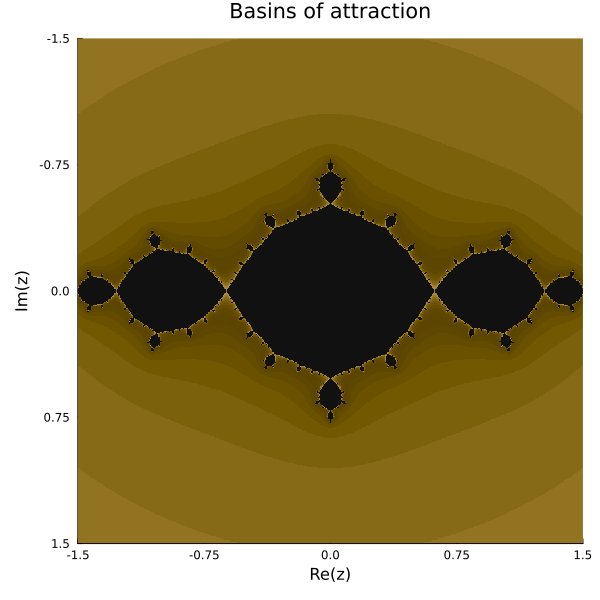
\includegraphics[width=0.55\textwidth]{figures/basins_z2m1.png}
  \caption{Retrato de cuencas de $f(z)=z^2-1$ generado con \fn{basin\_portrait}.
           La región coloreada es la cuenca del punto fijo en $\infty$.
           La zona negra no indica divergencia: corresponde a puntos
           cuya órbita converge al 2-ciclo $\{0,-1\}$,
           invisible para un algoritmo que solo busca puntos fijos.}
  \label{fig:basins_z2m1}
\end{figure}

Para revelar esa zona negra se usa \fn{basin\_portrait\_pcycle}, que detecta
convergencia a ciclos de periodo~$p$.
Fijando $p=2$, cada punto se clasifica según el elemento del 2-ciclo al que
su órbita se acerca primero, y los dos componentes del ciclo reciben un único
color de grupo (figura~\ref{fig:pcycle_z2}).

\begin{lstlisting}[caption={Cuencas del 2-ciclo de $f(z)=z^2-1$.}]
using RiemannBasins

num = complex([-1.0, 0.0, 1.0])   # z^2 - 1
den = complex([1.0])               # denominador = 1

# Paso 1: solo se ven cuencas de puntos fijos; el 2-ciclo aparece en negro
basin_portrait(num, den; bands = 8.0)

# Paso 2: basin_portrait_pcycle revela la cuenca del 2-ciclo
basin_portrait_pcycle(num, den, 2; bands = 8.0)
\end{lstlisting}

La función $f^2(z)=(z^2-1)^2-1$ tiene seis puntos fijos en $\Puno$
(cuatro finitos más $\infty$, siendo $\infty$ ya punto fijo de~$f$).
\fn{basin\_portrait\_pcycle} agrupa los dos componentes de Fatou del 2-ciclo
en un único color, independientemente de cuál de los dos elementos alcanza
primero la órbita.

\begin{figure}[ht]
  \centering
  % Comando: basin_portrait_pcycle(complex([-1.0,0.0,1.0]), complex([1.0]), 2;
  %          bands=8.0, savepath="figures/pcycle_z2.png")
  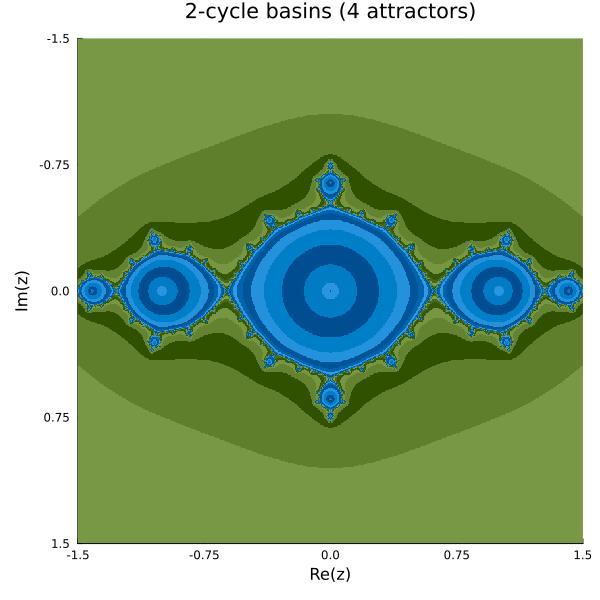
\includegraphics[width=0.55\textwidth]{figures/pcycle_z2.png}
  \caption{Cuencas del 2-ciclo $\{0,-1\}$ para $f(z)=z^2-1$,
           generadas con \fn{basin\_portrait\_pcycle}.
           La zona negra de la figura~\ref{fig:basins_z2m1} aparece ahora
           coloreada como cuenca del ciclo; la frontera fractal
           refleja la simetría $z\mapsto -z$ de~$f$.}
  \label{fig:pcycle_z2}
\end{figure}

% ============================================================
\section{Ver las cuencas: una visualización matemáticamente fundada}
\label{sec:visualizacion}
% ============================================================

\subsection{El problema de la elección de colores}

La asignación de colores a las cuencas de atracción parece una decisión
estética, pero tiene implicaciones matemáticas y de comunicación
científica nada triviales.
Un conjunto de colores mal elegido puede hacer que dos cuencas parezcan
más similares de lo que son, o que la velocidad de convergencia sea
imposible de distinguir.
Más importante aún: un tercio de la población masculina presenta alguna
forma de daltonismo, y una visualización que dependa del rojo-verde —la
más habitual— resulta ilegible para esas personas.

El negro tiene un papel reservado: se asigna a los píxeles cuya órbita
no ha convergido a ningún atractor en el número máximo de iteraciones
fijado.
Estos puntos aproximan el \emph{conjunto de Julia} $\mathcal{J}(f)$
(sección~\ref{ssec:julia}): la frontera fractal que separa las cuencas.
Cuanto mayor es la resolución y el límite de iteraciones, más fiel es la
aproximación.
El negro no es un fallo del algoritmo sino información geométrica:
delimita visualmente la región de comportamiento caótico.

\subsection{El espacio de color LCHab}

En el espacio RGB, que usa el monitor, diferencias iguales en los
valores $(R,G,B)$ no corresponden a diferencias iguales en la percepción:
el amarillo puro $(255,255,0)$ es perceptualmente mucho más brillante
que el azul puro $(0,0,255)$, aunque ambos tienen la misma saturación
formal.
Si asignamos colores RGB arbitrarios a las cuencas, una de ellas
destacará sobre las demás por un efecto de longitud de onda, no por
ninguna propiedad dinámica~\cite{Zeileis2009}.

El espacio CIE $L^*a^*b^*$ (abreviado \emph{Lab}) fue diseñado por la
Comisión Internacional de Iluminación en 1976 para ser
\emph{perceptualmente uniforme}~\cite{Schanda2007}: diferencias iguales
en las coordenadas $L^*$, $a^*$, $b^*$ corresponden a diferencias
aproximadamente iguales en la percepción humana del color.
Un tratamiento completo de los modelos de apariencia del color puede
encontrarse en~\cite{Fairchild2013}.

Su versión cilíndrica, el espacio \emph{LCHab}, usa:
\begin{itemize}
  \item $L^*\in[0,100]$: luminosidad ($L^*=0$ negro, $L^*=100$ blanco).
  \item $C^*\geq 0$: croma o saturación ($a^*=C^*\cos H^*$,\;
        $b^*=C^*\sin H^*$).
  \item $H^*\in[0^\circ,360^\circ)$: ángulo de tono.
\end{itemize}

Para asignar colores a $N$ cuencas de atracción, partimos de un color
semilla $(L_0^*, C_0^*, H_0^*)$ y distribuimos los tonos uniformemente:
\[
  H_k^* = H_0^* + k\,\frac{360^\circ}{N+1}, \qquad k=1,\ldots,N,
\]
manteniendo fijos $L_0^*$ y $C_0^*=\max(C_{\text{semilla}},40)$.
Al conservar la luminosidad y la croma, todos los colores resultantes
son perceptualmente equivalentes en brillo y saturación, independientemente
del ángulo de tono.
Esto garantiza que ninguna cuenca destaque artificialmente sobre las
demás por un efecto de contraste luminoso.

\begin{figure}[ht]
  \centering
  \begin{subfigure}[b]{0.47\textwidth}
    \centering
    % basin_portrait(num3, den3; bands=8.0, colorblind=false)
    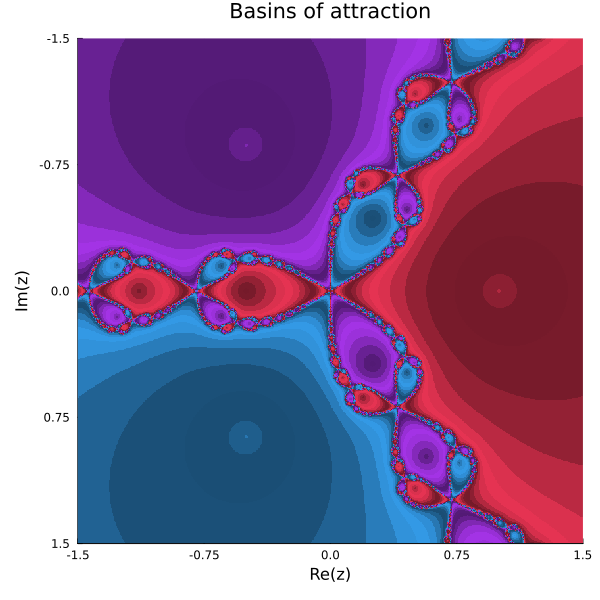
\includegraphics[width=\textwidth]{figures/newton_normal.png}
    \caption{Paleta LCHab estándar.}
  \end{subfigure}
  \hfill
  \begin{subfigure}[b]{0.47\textwidth}
    \centering
    % basin_portrait(num3, den3; bands=8.0, colorblind=true)
    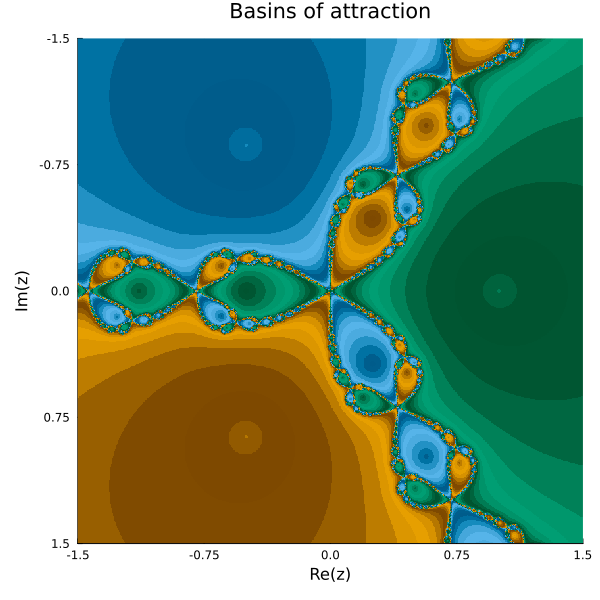
\includegraphics[width=\textwidth]{figures/newton_daltonico.png}
    \caption{Paleta Okabe--Ito (daltonismo).}
  \end{subfigure}
  \caption{Comparación de paletas para Newton en $z^3-1$.
           La paleta LCHab (izquierda) distribuye los tonos de forma
           equidistante en el espacio perceptual, maximizando el contraste
           entre cuencas para visión normal.
           La paleta Okabe--Ito~\cite{OkabeIto2008} (derecha) está
           diseñada para ser distinguible por personas con deuteranopía
           o protanopía, independientemente de los colores que aparezcan.
           Ambas conservan luminosidades equivalentes entre cuencas.}
  \label{fig:paletas}
\end{figure}

\subsection{Bandas de convergencia y conteo de iteraciones suavizado}

La velocidad con que una órbita se aproxima al atractor contiene
información geométrica rica.
Para visualizarla, usamos el \emph{conteo de iteraciones suavizado}.
Si la órbita de $z$ alcanza el atractor $\zeta$ tras $n$ iteraciones
con $|f^n(z)-\zeta|<\varepsilon$, definimos
\[
   \mu(z) = n - \frac{\log\log(|f^n(z)-\zeta|/\varepsilon)}{\log 2}
   \;\in\;\R_{\geq 0},
\]
que extiende el conteo entero a un valor real continuo y elimina la
discontinuidad que aparecería entre los niveles $n$ y $n+1$.
Modulamos entonces la luminosidad $L^*$ de cada píxel mediante:
\[
  L^*(z) = L_0^* + \Delta L\cdot\frac{1+\cos(2\pi\,b\,\tilde{\mu})}{2},
  \qquad \tilde{\mu}=\mu(z)/n_{\max},
\]
donde $b$ es el \emph{número de bandas} (parámetro del usuario) y
$\Delta L$ es la amplitud de la modulación.
El resultado son los anillos concéntricos visibles en la
figura~\ref{fig:bandas}: cada banda corresponde a una capa de puntos que tardan
aproximadamente el mismo número de iteraciones en converger.

Las bandas tienen además un significado geométrico: cerca del conjunto
de Julia $\mathcal{J}(f)$, las órbitas convergen más lentamente
—el valor $\mu(z)$ crece— y las bandas se comprimen hacia la frontera
fractal.
Con suficientes bandas, la imagen revela la estructura de
$\mathcal{J}(f)$ sin necesidad de calcularla directamente: las franjas
se aprietan precisamente donde la dinámica se vuelve más compleja.

\begin{figure}[ht]
  \centering
  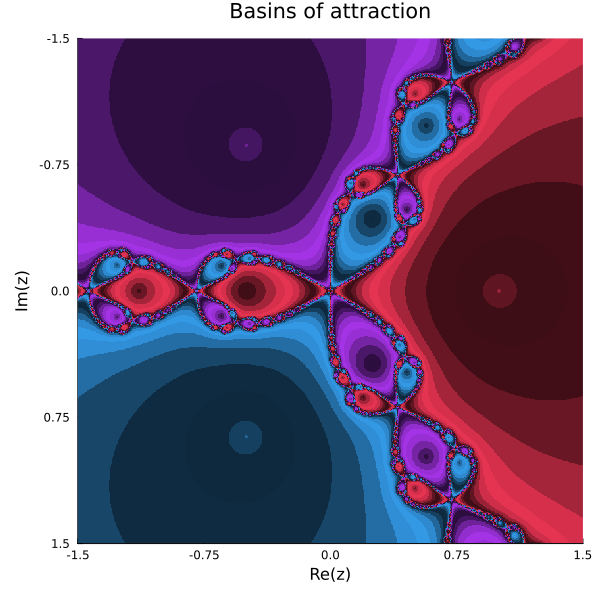
\includegraphics[width=0.60\textwidth]{figures/newton_bands.png}
  \caption{Efecto del bandeo en la visualización de Newton para $z^3-1$.
           La modulación de la luminosidad $L^*$ crea anillos concéntricos
           que revelan la velocidad de convergencia hacia cada atractor.
           Parámetro $b=8$ bandas.
           Generado con \pkg{RiemannBasins.jl}.}
  \label{fig:bandas}
\end{figure}

\subsection{El paquete \pkg{RiemannBasins.jl}}

Todas las figuras de este artículo han sido generadas con el paquete
\pkg{RiemannBasins.jl}~\cite{RiemannBasins2026}, escrito en Julia.
Las funciones racionales se especifican mediante listas de coeficientes
en coordenadas homogéneas, y la iteración se realiza directamente en
$\Puno$ para evitar los problemas de cancelación numérica cerca del
infinito.
Un ejemplo mínimo:

\begin{lstlisting}[caption={Retrato de cuencas para Newton en $z^3-1$ con visualización en las dos cartas de $\Puno$.}]
using RiemannBasins

# Numerador y denominador de N(z) = (2z^3+1)/(3z^2)
# Coeficientes en orden ascendente [a_0, a_1, ..., a_n]:
num = complex([1.0, 0.0, 0.0, 2.0])   # 1 + 2z^3 = 2z^3 + 1
den = complex([0.0, 0.0, 3.0, 0.0])   # 3z^2

# Retrato de cuencas en la carta estandar
basin_portrait(num, den; bands = 8.0)

# Retrato en las dos cartas estereograficas
two_chart_portrait(num, den; bands = 8.0)

# Superficie 3-D con GLMakie (requiere: using GLMakie)
basin_relief_3d_makie(num, den; bands = 50.0, relief_scale = 0.01)

# Cuencas de ciclos de periodo p (p = 2 en el ejemplo)
basin_portrait_pcycle(num, den, 2; bands = 8.0)
\end{lstlisting}


% ============================================================
\section{Recapitulación y caminos abiertos}
\label{sec:conclusion}
% ============================================================

Hemos mostrado que el espacio proyectivo $\Puno$ es el dominio natural
para la dinámica de iteración de funciones racionales.
Trabajar en coordenadas homogéneas, en lugar de en $\C$ con el infinito
tratado como caso especial, tiene consecuencias concretas: el
Teorema~\ref{teo:puntosfijos} da exactamente $d+1$ puntos fijos, la
segunda carta estereográfica hace visible la cuenca del infinito, y la
simetría global del sistema queda de manifiesto.

Los ejemplos clásicos —Newton, Halley, la familia $z^2+c$— ilustran
que distintas estrategias de iteración producen estructuras globalmente
distintas en~$\Puno$, y que la geometría de las cuencas en la segunda
carta completa el cuadro que la carta afín estándar deja parcialmente
oculto.
La elección de colores en el espacio LCHab garantiza que todas las
cuencas sean igualmente visibles y que la velocidad de convergencia
quede codificada en una señal visual continua.

Los cinco tipos de componentes periódicas del teorema de
Fatou--Sullivan (figura~\ref{fig:fatou-tipos}) no aparecen todos en
los ejemplos anteriores.
Los tipos~(i) y~(ii) —cuencas de atractores fijos y de ciclos— están
bien representados.
Las \emph{cuencas parabólicas} (tipo~iii) aparecen cuando el
multiplicador es una raíz de la unidad; el ejemplo más sencillo es
$f(z)=z^2+\tfrac{1}{4}$, cuyo punto fijo $z=\tfrac{1}{2}$ tiene
multiplicador~$\lambda=1$.
Los \emph{discos de Siegel} y los \emph{anillos de Herman}
(tipos~iv y~v) exigen que el multiplicador sea $e^{2\pi i\alpha}$ con
$\alpha$ irracional sujeto a condiciones aritméticas muy finas
(los denominados \emph{números de Brjuno}): son los tipos más raros,
pero visualmente los más sorprendentes, pues la dinámica rota sin
converger y sin divergir.
Visualizar estos tres tipos adicionales —para lo cual habría que
adaptar el algoritmo de convergencia a cada caso— queda como una
línea de desarrollo pendiente del paquete y como invitación al lector
a buscar ejemplos en la literatura.

Una extensión inmediata del paquete es la detección automática del
período mínimo del ciclo atractor, evitando que el usuario especifique
$p$ a priori: iterar $f, f^2, f^3,\ldots$ hasta detectar coincidencia
es computacionalmente factible para los grados habituales.
Esto permitiría visualizar familias completas como $z^2+c$ sin
necesidad de conocer de antemano el diagrama de bifurcación.

Una dirección más ambiciosa es pasar de una sola función a
\emph{dos}: dadas $f$ y $g$ racionales, el semigrupo
$\langle f,g\rangle$ generado por sus composiciones posee su propio
conjunto de Fatou y su propio conjunto de Julia, cuya teoría fue
iniciada por Hinkkanen y Martin~\cite{HinkkanenMartin1996}.
Visualizar las cuencas de este semigrupo en $\Puno$ —¿qué regiones
convergen bajo qué composiciones?— abriría una ventana a la dinámica
comparada de métodos numéricos: ¿qué ocurre en el plano complejo
cuando se alterna Newton y Halley sobre el mismo polinomio?

% ============================================================
\section*{Agradecimientos}
% ============================================================

V.~Álvarez Aparicio y M.~T.~Rivas Rodríguez han contribuido a la
redacción del texto, a la revisión estilística, a la búsqueda y
verificación de referencias bibliográficas, y a la mejora general
de la exposición.
El paquete \pkg{RiemannBasins.jl} y el presente artículo se
desarrollaron con asistencia del modelo de lenguaje Claude
(Anthropic), que colaboró en la discusión de enfoques,
la estructuración de contenidos y la elaboración de las figuras
TikZ.

Los tres autores son miembros del Grupo de Investigación
\emph{Geometría, Topología e Historia de las Matemáticas},
que cuenta con el apoyo de la ayuda REGI25/61.
El presente artículo no ha contado con financiación específica.

% ============================================================
\begin{thebibliography}{9}
% ============================================================

\bibitem{HinkkanenMartin1996}
A.~Hinkkanen e~I.~N.~Martin,
«The dynamics of semigroups of rational functions I»,
\textit{Proc.\ London Math.\ Soc.} \textbf{73} (1996), 358--384.

\bibitem{Milnor2006}
J.~Milnor,
\textit{Dynamics in One Complex Variable},
3.ª~ed., Princeton University Press, Princeton, 2006.

\bibitem{Beardon1991}
A.~F.~Beardon,
\textit{Iteration of Rational Functions},
Springer-Verlag, Nueva York, 1991.

\bibitem{CarlsonEtAl1994}
N.~Carlson, D.~Mandell y J.~F.~Epperson,
«Newton's method for the complex cube roots of unity»,
\textit{Amer.\ Math.\ Monthly} \textbf{101} (1994), 645--648.

\bibitem{OkabeIto2008}
M.~Okabe e~I.~Ito,
«Color universal design (CUD): how to make figures and presentations
that are friendly to colorblind people»,
\textit{J.\ Jap.\ Assoc.\ Human Genetics} \textbf{53} (2008), 1--7.

\bibitem{Zeileis2009}
A.~Zeileis, K.~Hornik y P.~Murrell,
\guillemotleft Escaping RGBland: Selecting Colors for Statistical
Graphics\guillemotright,
\textit{Comput.\ Statist.\ Data Anal.}\ \textbf{53} (2009),
3259--3270.

\bibitem{Schanda2007}
J.~Schanda (ed.),
\textit{Colorimetry: Understanding the CIE System},
Wiley, Hoboken, 2007.

\bibitem{Fairchild2013}
M.~D.~Fairchild,
\textit{Color Appearance Models},
3.ª~ed., Wiley, 2013.

\bibitem{RiemannBasins2026}
L.~J.~Hernández~Paricio,
\textit{RiemannBasins.jl: visualización de cuencas de atracción de
funciones racionales en la esfera de Riemann},
Universidad de La Rioja, 2026.
Disponible en: \url{https://github.com/luhernan/RiemannBasins.jl}


\bibitem{Jones1987}
G.~A.~Jones y D.~Singerman,
\textit{Complex Functions: An Algebraic and Geometric Viewpoint},
Cambridge University Press, Cambridge, 1987.

\bibitem{Miranda1995}
R.~Miranda,
\textit{Algebraic Curves and Riemann Surfaces},
American Mathematical Society, Providence, 1995.

\bibitem{Needham1997}
T.~Needham,
\textit{Visual Complex Analysis},
Oxford University Press, Oxford, 1997.

\end{thebibliography}

\end{document}
